\documentclass[10pt, paper=letter]{scrartcl} % tabellarischer Lebenslauf
\usepackage[american]{babel}
\RequirePackage{makecmds}

\usepackage[utf8]{inputenc}
\usepackage[T1]{fontenc}
\usepackage[letterpaper,left=2cm, right=2cm, top=2.5cm, bottom=2cm]{geometry}

\usepackage{currvita,graphicx,microtype,csquotes,xcolor,doipubmed,charter,fancyhdr,lastpage,soul}

%\usepackage[defaultsans,oldstyle,scale=0.95]{opensans}
\usepackage[default]{FiraSans}
%\renewcommand{\familydefault}{\sfdefault}
\renewcommand{\familydefault}{\rmdefault}

\usepackage[bookmarks,hidelinks]{hyperref}
\usepackage[hyphenbreaks]{breakurl}

\usepackage[shortcuts]{extdash} % hyphenation rules for dashes: - : \-/(no hyphenation: \=/) | -- : \-- (\==) | --- : \--- (\===)  

%\date{April 15, 2019}
%\cvplace{Thunder Bay, ON}

\pagestyle{fancy}
\renewcommand{\headrulewidth}{0pt}
\lhead{\color{gray}\textsf{\MakeUppercase{Curriulum vit\ae}}}
\chead{}
\rhead{\color{gray}\textsf{Tobias Stephan}}
%\rhead{}
%\cfoot{\thepage/11}
\cfoot{\color{gray}\textsf{\thepage\ of \pageref{LastPage}}}

\renewcommand{\thefootnote}{\fnsymbol{footnote}} 

\setkomafont{section}{\Large\scshape\MakeLowercase}
\setkomafont{subsection}{\large}


\begin{document}

\addcontentsline{toc}{chapter}{Curriculum Vitae}

\begin{cv}{\textsf{Dr Tobias Stephan}}
    \medskip
    % \noindent\begin{minipage}{.74\linewidth}%
    %\medskip
    \noindent  Postdoctoral associate\smallskip \\
    Lakehead University\\
    Department of Geology\\
    Thunder Bay, ON, Canada\smallskip \\
    %Earth Sciences, Calgary, AB, T2N 1N4 \smallskip \\
    \noindent Email: \href{mailto:tstephan@lakeheadu.ca}{tstephan@lakeheadu.ca}\\
    Website: \url{https://tobiste.github.io/}\\
    ORCID: \href{https://orcid.org/0000-0002-9290-014X}{0000-0002-9290-014X}
    % \bigskip
    % \end{minipage}%
    % \hfill
    % \begin{minipage}{.24\linewidth}%
    % \raggedleft
    %   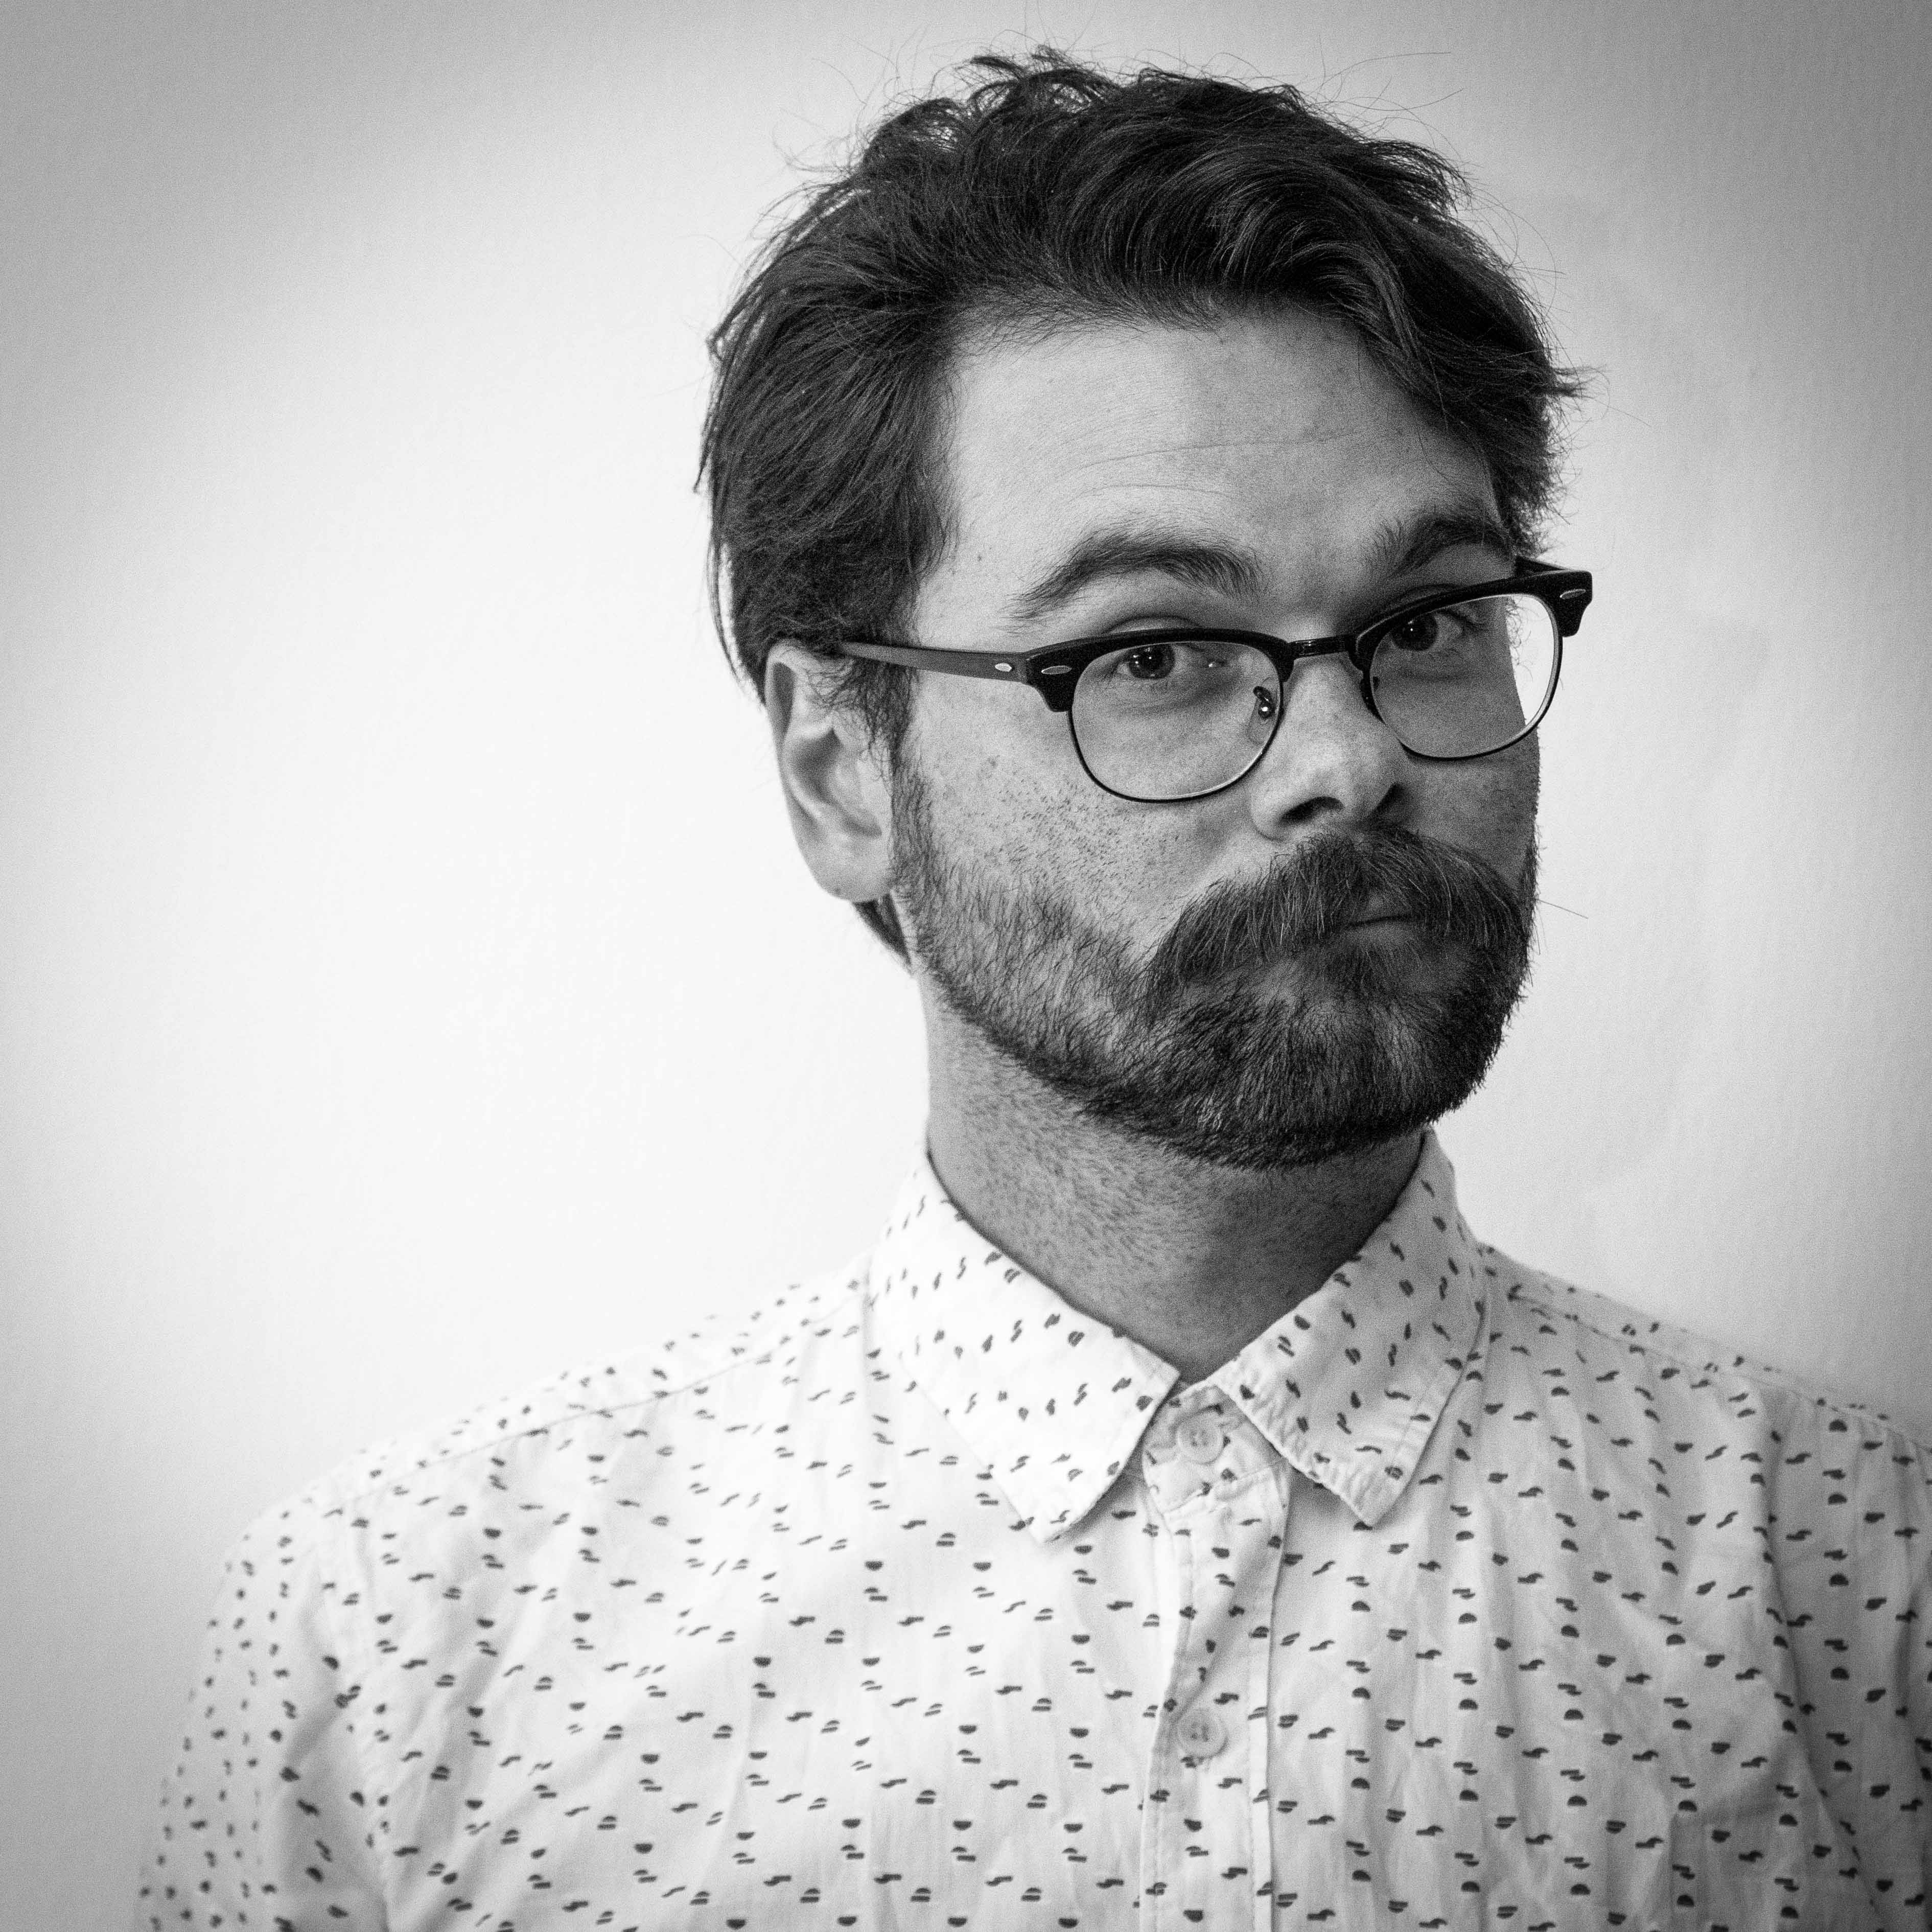
\includegraphics[width = \linewidth]{tobi.jpg}
    % \end{minipage}%

    %\medskip

    % \noindent {\large \textbf{Research interests}}
    % \begin{itemize}\setlength\itemsep{-0.2em}
    %     \item Convergent tectonics
    %     \item Analysis of large-scale patterns of stress and strain fields and their link to tectonic forces
    %     \item Analysis of plate motion
    %     \item Plate tectonic reconstructions
    %     \item Structural analysis of polyphase brittle and ductile deformation
    %     \item Sedimentary provenance analysis
    %     \item Exloring and analysing large geo-datasets using modern statistical tools
    %     \item Paleozoic tectonics of the Variscides
    %     \item Cenozoic tectonics of central Europe and Canadian Cordillera
    % \end{itemize}
    % 
    % 
    % \smallskip

    \section{Education}
    \begin{cvlist}{}
        \item[2019/03] \textbf{Doctor of Philosophy (PhD)} in \enquote{Geology}\\ \textit{Technische Universit\"at Bergakademie Freiberg, Germany}
        \begin{itemize}\setlength\itemsep{-0.5em}
            \item Thesis: \enquote{Paleogeographic and Structural Control on the Arcuate Variscan
                      Belt}
            \item Supervisors: Dr Uwe Kroner (Technische Universit\"at Bergakademie Freiberg) and
                  Prof Dr Rolf L. Romer (Geoforschungszentrum Potsdam)
                  %\item Grade: summa cum laude (\enquote{with highest honors}, numerical grade < 1.0)
        \end{itemize}
        \item[2013/09] \textbf{Master of Science (MSc)} in \enquote{Geosciences} (major: Tectonics and Geochronology)\\
        \textit{Technische Universit\"at Bergakademie Freiberg, Germany}
        \begin{itemize}\setlength\itemsep{-0.5em}
            \item Thesis: \enquote{Variscan Tectonics of the Schwarzburg unit (Central European
                      Variscides): From a transform plate boundary zone to an orogenic wedge}
            \item Supervisor: Dr Uwe Kroner (Technische Universit\"at Bergakademie Freiberg)
                  %\item Grade: 1.1
        \end{itemize}
        \item[2010/09] \textbf{Bachelor of Science (BSc)} in \enquote{Geology and Mineralogy}\\
        \textit{Technische Universit\"at Bergakademie Freiberg, Germany}
        \begin{itemize}\setlength\itemsep{-0.5em}
            \item Thesis: \enquote{Structural geology and sedimentology of the Tanne Greywacke
                      Zone, Harz Mts., Germany}
            \item Supervisor: Dr Uwe Kroner (Technische Universit\"at Bergakademie Freiberg)
                  %\item Grade: 1.3
        \end{itemize}
    \end{cvlist}

    \section{Professional Experience}
    \begin{cvlist}{}
    %\item[since 2025/08]  \textbf{Assistant Professor}\\ \textit{Lakehead University,
    %        Department of Geology, Thunder Bay, ON, Canada}
        \item[since 2023/04] \textbf{Postdoctoral associate}\\ \textit{Lakehead University,
            Department of Geology, Thunder Bay, ON, Canada}\\ Project: \enquote{Structure,
            petrology, geochemistry, and geochronology of the Moss Lake Au deposit,
            Northern Ontario, Canada} --- NSERC Alliance Grant\\ Advisors: Dr Noah J.
        Phillips, Dr Peter Hollings
        
        \item[since 2024/09] \textbf {Lecturer}\\ \textit{Lakehead University, Department of
            Geology, Thunder Bay, ON, Canada}       

        \item[2020/12--2022/11] \textbf{Postdoctoral associate} (DFG Research Fellow)\\
        \textit{University of Calgary, Geo- and Thermochronology Research Group, Department of Geoscience, Calgary, AB, Canada}\\
        Project:
        \enquote{Developing a statistical approach to analyze large paired geo-thermochronological datasets with an application to the Canadian Cordilleras} --- \href{https://gepris.dfg.de/gepris/projekt/439621066?language=en}{DFG Research Fellowship}\\
        Advisor: Dr Eva Enkelmann

        \item[2020/03--2020/11] \textbf{Postdoctoral associate}\\
        \textit{
            Friedrich-Alexander-Universit\"at Erlangen-N\"urnberg, Geozentrum Nordbayern, \mbox{Erlangen}, Germany} \\ Project: \enquote{Integrated geophysical–structural–kinematic analysis of the fault patterns in Northern Bavaria} --- LfU Bayern \& ERDF\\
        Advisors: Dr Daniel Koehn, Dr Harald Stollhofen

        \item[2019/09--2019/12] \textbf{Research assistant}\\
        \textit{Technische Universit\"at Bergakademie Freiberg, Institute for Computer Sciences, Freiberg, Germany}

        \item[2014--2018] \textbf{Research assistant}\\
        \textit{Technische Universit\"at Bergakademie Freiberg, Institute for Geology}
        \\ Projects: \enquote{Developing a method for three dimensional forecasting of covered mineral deposits on the example of the Erzgebirge} --- BMBF ZIM and \enquote{Granite related mineralization of strategic metals (GEM) – conditions of mineralization and search criteria for hidden ore bodies} --- \href{https://www.gfz-potsdam.de/en/section/inorganic-and-isotope-geochemistry/projects/prohydrogen-more-mofette-research-prosalz-gramm-sugar-gem-amrep-halmahera-gogaf-irup-spp-sample-ketzin-co2-cosanostra-inkaba-yeafrica-dafgas/gem/bmbf-r4-gem}{BMBF~r4}
        %         \begin{itemize}\setlength\itemsep{-0.5em}
        %         \item statistical analysis of large datasets of detrital zircon U\--Pb ages
        %         \item pre-Pangean paleogeography of northern Gondwana 
        %         \item structural and tectonic research on the arcuate shape of the Variscan Orogen
        %         \item field work in Germany, SW Britain, NW Iberia
        %         \item trigger mechanisms of swarm earthquakes in East Germany
        %         \end{itemize} 		
        \item[2014/01--2014/06] \textbf{Geologist}\\
        \textit{Beak Consultants GmbH (Germany\,/\,Tanzania)}\\
        Field work in Tanzania, compilation for metallogenic database of Tanzania, GIS training to the staff of the Geological Survey of Tanzania, Dodoma, Tanzania
        %             \begin{itemize}\setlength\itemsep{-0.5em}
        %             \item field work in Tanzania, evaluating economic potential of Central Tanzania
        %             \item data entry for metallogenic database \href{https://www.gmis-tanzania.com/}{GMIS}
        %             \item digitization of geological maps of Tanzania
        %             \item ArcGIS training to the staff of the Geological Survey of Tanzania (Dodoma)
        %             \end{itemize}		
        \item[2009--2013] \textbf{Lab assistant}\\
        \textit{Technische Universit\"at Bergakademie Freiberg, Institute for Geology}\\ Rock processing and mineral separation for geochronological and thermochronological analyses (Ar\--Ar, fission track, U\--Pb)
        %             \begin{itemize}
        %             \item rock processing and mineral separation for geochronological analyses (Ar\--Ar, fission track, U\--Pb)
        %             \end{itemize}
        \item[2011/07--2011/09] \textbf{Teaching and research assistant (IAESTE student exchange)}\\
        \textit{Mongolian University of Science and Technology, Ulaanbaator, Mongolia}\\ Field work in ophiolitic sequences of Western Mongolia focusing on local and regional scale structures

        \item[2007/05--2007/06] \textbf{Student internship}\\
        \textit{GFZ German Research Center for Geosciences  Potsdam, Department for Geomagnetism, Potsdam, Germany}\\
        Contribution to the \href{http://isdc.gfz-potsdam.de/igrf-declination-calculator/}{IGRF Declination Calculator}, an online software for estimating the magnetic field declination, inclination, and intensity for any location on Earth and times since 1990
    \end{cvlist}

    \section{Teaching Experience}
    \subsection{Previous taught courses}

    \begin{cvlist}{}
        \item[2025/01--2025/04] Geology Case Studies\\
        \textit{Lakehead University, Department of Geology, Thunder Bay, ON, Canada}\\
        Course level: undergraduate | lecture hours per week: 3
        \item[2024/09--2024/12] Structural Geology \& Tectonics\\
        \textit{Lakehead University, Department of Geology, Thunder Bay, ON, Canada}\\
        Course level: undergraduate |  lecture hours per week: 3
        \item[2023/10] Short course: \enquote{Plate motion and deformation of the lithosphere} (1 week)\\
        \textit{Department of Geology, Technische Universit\"at Bergakademie Freiberg, Germany}
        Course level: postgraduate-graduate | number of students: 20 | lecture hours per week: 20
        \item[2022/09] Short course \enquote{Programming with R --- A Beginners’ Guide for Geoscientists} (1 week)\\
        \textit{University of Calgary, Department of Geoscience, Calgary, AB, Canada}\\
        Course level: graduate | number of students: 8 | lecture hours per week: 12
        \item[2022/01] Guest lecture: \enquote{Structural geology}\\
        \textit{University of Calgary, Department of Geoscience, Calgary, AB, Canada}\\
        Course level: undergraduate | number of students: 23 | lecture hours per week: 1
        \item[2019/09--2019/12] 3D Modeling in Earth Sciences\\
        \textit{Institute for Computer Sciences, Technische Universit\"at Bergakademie Freiberg, Germany}\\
        Course level: undergraduate | number of students: 20 | lecture hours per week: 4
        \item[2017/10--2018/03] Specific Topics of Applied Geomodelling\\
        \textit{Department of Geophysics and Geoinformatics, Technische Universit\"at Bergakademie Freiberg, Germany}\\
        Course level: undergraduate | number of students: 20 | lecture hours per week: 2
        \item[2015--2018] Teaching assistant for field course \enquote{Strucutral Geology}\\
        \textit{Department of Geology, Technische Universit\"at Bergakademie Freiberg, Germany}
        \item[2014/01--2014/05] Digital maps and GIS courses\\
        \textit{Geological Survey of Tanzania, Dodoma, Tanzania}
        \item[2011/07--2011/09] Teaching and field work assistant during geological mapping courses in Khangai Mnts., Mongolia\\
        \textit{Mongolian University of Science and Technology, Ulaanbaator, Mongolia}\\
        Course level: undergraduate | number of students: 40
    \end{cvlist}

    % \newpage
    \subsection{Student Mentorship}
    \begin{cvlist}{Graduate level:}
        \item[4] Tiitto, H. \enquote{The Quetico Fault System: Insights into crustal-scale structures within the brittle-ductile regime}\\
        Degree: Master of Science. Started: 2024/06, \textit{Lakehead University, Thunder Bay}
        \item[3] Perez, A. \enquote{Petrology and Geochemistry of the western
            Shebandowan Greenstone Belt (Superior Province, Northern Ontario, Canada)}\\
        Degree: Master of Science.
        Started: 2023/04, \textit{Lakehead University, Thunder Bay, Canada}
        \item[2] Nwakanma, M. \enquote{Alteration and mineral paragenesis of the Moss Lake gold deposit (Shebandowan Greenstone Belt, Superior Province, Northern Ontario, Canada)}\\
        Degree: Master of Science.
        Started: 2023/04, \textit{Lakehead University, Thunder Bay, Canada}

        %\item[2] Unger, A., \enquote{...}\\
        %Degree: Master of Science. Completed: 2021, \textit{Technische Universität Bergakademie Freiberg, Germany}

        \item[1] Müller, F. \enquote{Tectonic 3D model of the Berga Antiform, Saxothuringian Zone, Germany}\\
        Degree: Master of Science.
        Completed: 2018/04/30, \textit{Technische Universität Bergakademie Freiberg, Germany}
    \end{cvlist}

    % put in chronological order
    \begin{cvlist}{Undergraduate level:}
        \item[7] Tiitto, H. \enquote{Anatomy of an Archean terrane boundary:
            Structural analysis of the boundary between the Quetico and Wawa Subprovinces
            (Superior Province)}\\
        Degree: Bachelof of Honours. Started: 2023/08, \textit{Lakehead University, Thunder
            Bay, Canada}

        \item[6] Lippke, H. \enquote{Geology of Cornwall}\\
        Degree: Bachelor of Science. Completed: 2018/03/12, \textit{Technische Universität Bergakademie Freiberg, Germany}

        \item[5] Trilsch, F. \enquote{3D model of the Eibenstock Granite}\\
        Degree: Bachelor of Science. Completed: 2018, \textit{Technische Universität Bergakademie Freiberg, Germany}

        \item[4] Hartmann, C. \enquote{Variscan tectonics of Devonian synorogenic sediments in Northwestern Cornwall\,/\,UK}\\
        Degree: Bachelor of Science. Completed: 2017/12/19, \textit{Technische Universität Bergakademie Freiberg, Germany}

        \item[3] Miebach, I. \enquote{Geology of the Ollo de Sapo formation of Iberia --- A compilation of tectonic, geochronological, and geochemical data}\\
        Degree: Bachelor of Science. Completed: 2017/07/20, \textit{Technische Universität Bergakademie Freiberg, Germany}

        \item[2] Unger, A. \enquote{Tectonics of low-grade metasedimentary rocks of the Vogtland near Kling\-en\-thal}\\
        Degree: Bachelor of Science. Completed: 2016/11/21, \textit{Technische Universität Bergakademie Freiberg, Germany}

        \item[1] Roethe, R. \enquote{Structural geology and petrography of the Eibenstock granite}\\
        Degree: Bachelor of Science. Completed: 2014/09/25, \textit{Technische Universität Bergakademie Freiberg, Germany}
    \end{cvlist}

    \subsection{Additional Training}
    \begin{cvlist}{}
        \item[since 2024] Organization of the weekly \textit{Structural Geology Seminar} at
        Lakehead University
        \item[2021--2022] Organization of the weekly \textit{Thermochronology Seminar} at the University of Calgary
        \item[2018] Organization and field trip co-leader, \textit{Variscan tectonics of Cornwall, SE Britain}
        \item[2016] Organization of the international workshop \textit{Late Paleozoic tectonic and magmatic evolution of the Erzgebirge Complex, Germany}, assistant and field trip co-leader
    \end{cvlist}

    %\newpage 
    \section{Publications}
    \subsection{Peer-reviewed articles}
    \setul{1pt}{.4pt}% set underline 1pt below contents
    \begin{cvlist}{}
        %\item[total times cited:] 267\footnote[1]{Web of Science} (362\footnote[2]{Google Scholar})
        % \item[h-index:] 6\footnotemark[1] (7\footnotemark[2])
        \item[-] \ul{Stephan, T.}  Phillips, N., Tiitto, H., and Hollings, P. \enquote{Going with the flow --- Changes of  Vorticity Controls Gold Enrichment in Archean Shear Zones (Shebandowan Greenstone Belt, Superior Province, Canada)}. submitted to \textit{Structural Geology} in February 2025.
        
        %\item[-] Duschl, F., \ul{Stephan, T.}, K\"ohler, S., Drews, M., Koehn, D., and Stollhofen, H. \enquote{How continents (de-)form: A paleostress chart for Central Europe}. submitted to \textit{Geology} in August 2024.
        \item[-] \ul{Stephan, T.}, and Enkelmann, E. \enquote{All Aligned on the Western Front of North America? Analyzing the Stress Field in the Northern Cordillera}. submitted to \textit{Tectonics} in July 2024.

        \item[14] Padgett, J., Enkelmann, E., Kellett, D., Moynihan, D., and \ul{Stephan, T.} (2025): \enquote{Cenozoic faulting in the Upper Hyland River Valley, Southeastern Yukon: A thermochronological perspective}. \textit{Canadian Journal of Earth Sciences}. \doi{10.1139/cjes-2024-0147}.
        
        \item[13] Schaeben, H., Kroner, U., and \ul{Stephan, T.} (2024): \enquote{Mathematical Fundamentals of Spherical Kinematics of Plate Tectonics in Terms of Quaternions}. \textit{Mathematical Models and Methods in Applied Sciences} 47(6). pp. 4469--4496. \doi{10.1002/mma.9823}

        \item[12] \ul{Stephan, T.}, Enkelmann, E., and Kroner, U. (2023): \enquote{Analyzing the horizontal orientation of the crustal stress adjacent to plate boundaries}. \textit{Scientific Reports} 13:15590. \doi{10.1038/s41598-023-42433-2}.
        %
        \item[11] Járóka, T.,  Pfänder, J.\,A., Seifert, T., Hauff, F., Sperner, B., Staude, S., \ul{Stephan, T.}, and Schulz, B. (2023): \enquote{Age and petrogenesis of Ni-Cu-(PGE) sulfide-bearing gabbroic intrusions in the Lausitz Block, northern Bohemian Massif (Germany/Czech Republic)}. \textit{Lithos} 444--445:107090. \doi{10.1016/j.lithos.2023.107090}
        %
        \item[10] Kroner, U., Romer, R.\,L., and \ul{Stephan, T.} (2023): \enquote{Die Rekonstruktion von relativen Plattenbewegungen aus dem paläozoischen Deformationsmuster der kontinentalen Kruste}. \textit{Zeitschrift der Deutschen Gesellschaft für Geowissenschaften (J. Appl. Reg. Geol.)} 174 (3). pp. 491--519. \doi{10.1127/zdgg/2023/0365}
        %
        \item[9] K\"ohler, S., Duschl, F., Fazlikhani, H., Koehn, D., \ul{Stephan, T.}, and Stollhofen, H. (2022): \enquote{Reconstruction of cyclic Mesozoic-Cenozoic stress development in SE Germany using fault-slip and stylolite inversion}. \textit{Geological Magazine} 159 (11--12). pp. 2323--2345.\newline
        \doi{10.1017/S0016756822000656}
        %
        \item[8] Kroner, U., \ul{Stephan, T.}, and Romer, R.\,L. (2022): \enquote{Paleozoic orogenies and relative plate motions at the sutures of the Iapetus-Rheic Ocean}. In Y.\,D. Kuiper, J.\,B. Murphy, R.\,D. Nance, R.\,A. Strachan, and M.\,D. Thompson (Eds.), \textit{New Developments in the Appalachian-Caledonian-Variscan Orogen}. Geological Society of America. \doi{10.1130/2021.2554(01)}
        %
        \item[7] Schaeben, H., Kroner, U., and \ul{Stephan, T.} (2021): \enquote{Euler Poles of Tectonic Plates}. In B.\,S. Daza Sagar, Q. Cheng, J. McKinley, and F. Agterberg (Eds.), \textit{Encyclopedia of Mathematical Geosciences. Encyclopedia of Earth Sciences Series. Springer Nature} Switzerland AG 2021. \doi{10.1007/978-3-030-26050-7\_435-1}
        %
        \item[6] Caracciolo, L., Ravid\`a, D.\,C.\,G., Chew, D., Jan{\ss}en, M., L\"unsdorf, N.\,K., Heins, W.\,A., \ul{Stephan, T.}, and Stollhofen, H. (2021): \enquote{Reconstructing environmental signals across the Permian-Triassic boundary in the SE Germanic Basin: A Quantitative Provenance Analysis (QPA) approach}. \textit{Global and Planetary Change}, 206:103631.  \doi{10.1016/j.gloplacha.2021.103631}
        \item[5] Kroner, U., \ul{Stephan, T.}, Romer, R.\,L., and Roscher, M. (2020): \enquote{Paleozoic plate kinematics during the Pannotia--Pangaea supercontinent cycle}. \textit{Geological Society, London, Special Publications} 503, SP503-2020-15. \doi{10.1144/SP503-2020-15}
        %
        \item[4] \ul{Stephan, T.}, Kroner, U., Romer, R.\,L., and R\"osel, D. (2019): \enquote{From a bipartite Gondwana shelf to the arcuate Variscan belt: The Early Paleozoic evolution of northern Peri-Gondwana}. \textit{Earth-Science Reviews} 192, pp. 491--512. \doi{10.1016/j.earscirev.2019.03.012}
        %
        \item[3] Heinicke, J., \ul{Stephan, T.}, Alexandrakis, C., Buske, S., and Gaupp, R. (2019): \enquote{Alteration as possible cause for transition from brittle failure to aseismic slip: the case of the NW-Bohemia\,/\, Vogtland earthquake swarm region}. \textit{Journal of Geodynamics} 124, pp. 79--92. \doi{10.1016/j.jog.2019.01.010}
        %
        \item[2] \ul{Stephan, T.}, Kroner, U., and Romer, R.\,L. (2018): \enquote{The pre-orogenic detrital zircon record of the Peri-Gondwanan crust}. \textit{Geological Magazine} 156\,(2), pp. 281--307.\newline
        \doi{10.1017/s0016756818000031}.
        \href{https://www.cambridge.org/core/journals/geological-magazine/most-cited?searchWithinIds=277295E1DFDC1E4700796E746AE514CC&productType=JOURNAL_ARTICLE&pageSize=20&filters\%5BisCitedByMin\%5D=0&template=cambridge-core\%2Fjournal\%2Farticle-listings\%2Flistings-wrapper&displayNasaAds=false&showCitationNumbers=true&suppressArticleTypeGrouping=true&sort=platformMetadata.citationCount.crossRef\%3Adesc&filters\%5BdateYearRange\%5D\%5Bfrom\%5D=2017}{\textbf{Journal's most cited article since 2017}}
        %
        \item[1] \ul{Stephan, T.}, Kroner, U., Hahn, T., Hallas, P., and Heuse, T. (2016): \enquote{Fold\,/\,cleavage relationships as indicator for late Variscan sinistral transpression at the Rheno\-/Hercynian\--Saxo\-/Thuringian boundary zone, Central European Variscides}. \textit{Tectonophysics} 681, pp. 250--262. \doi{10.1016/j.tecto.2016.03.005}

        %\item[in prep] Stephan, T. and Enkelmann, E., \enquote{Statistical Analysis of the First-Order Intraplate Stress Field of Alaska and the Canadian Cordillera}. to be submitted to \textit{Tectonics} (December 2023).
        %\item Duschl, F., Stephan, T., K\"ohler, S., Drews, M., Koehn, D., and Stollhofen, H. \enquote{How continents (de-)form: A paleostress chart for Central Europe}. to be submitted to \textit{Geology} (December 2023).   
        %\item Stephan, T., Kroner, U., K\"ohler, S., Koehn, D., and Stollhofen, H., \enquote{Large-scale Stress Deflection Associated With Lithospheric Structural Inheritance of Western-Central Europe}. to be submitted to \textit{EGU: Solid Earth} (December 2023).
    \end{cvlist}

    %\newpage
    \subsection{Conference proceedings}
    \begin{cvlist}{} %\footnotetext{\textsf{only first authored contributions listed}}
         \item[42] Stephan, T., Tiitto, H., Nwakanma, M., Perez, A., Phillips, N. J., Hollings, P. N., and Flindell, P. (2025): Going with the flow --- Changes of Vorticity Control Gold Enrichment in Archean Shear Zones of the Shebandowan Greenstone Belt (Superior Province, Canada).  \textit{GAC-MAC 2025},  Ottawa, ON
         \item[41] Enkelmann, E. and Stephan, T. (2025): What drives Cenozoic to ongoing deformation in the Northern Cordillera? \textit{GAC-MAC 2025},  Ottawa, ON
        \item[40] Stephan, T. (2025): Does plate boundary obliquity predict interplate deformation? \textit{GAC-MAC 2025},  Ottawa, ON
        \item[39] Tiitto, H., Phillips, N., and Stephan, T. (2024): The Quetico Fault System: Insights into crustal-scale structures within the brittle-ductile regime. \textit{CTG Fall Field Trip},  Antigonish, Nova Scotia
        \item[38] Kroner, U. and Stephan, T. (2024): Kossmat’s zonation of the Central European basement in the light of the current knowledge. \textit{GeoSaxonia2024}, Dresden, GER
        \item[37] Stephan, T. (2024): Testing the link between plate boundary obliquity and interplate deformation. \textit{GSA 2024}, Anaheim, CA, USA
        \item[36] Enkelmann, E. and Stephan, T. (2024): Unveiling the Northern Cordilleran Puzzle: From the St. Elias to the Mackenzie Mountains. \textit{GSA 2024}, Anaheim, CA, USA
        \item[35] Kroner, U. and Stephan, T. (2024): Kossmat’s zonation of the Central European basement in the light of the current knowledge. \textit{GeoSaxonia 2024}, Dresden, Germany
        \item[34] Tiitto, H., Stephan, T., and Phillips, N. J. (2024): Anatomy of an Archean terrane boundary: Structural analysis of the boundary between the Quetico and Wawa Subprovinces (Superior Province). \textit{GAC-MAC-PEG 2024}, Brandon, MN
        \item[33] Stephan, T., Perez, A., Nwakanma, M., Phillips, N. J., Hollings, P. N., and Flindell, P. (2024): Chemical and structural constraints of shear-zone hosted gold mineralization from the Archean Shebandowan Greenstone Belt (Superior Craton, NW Ontario). \textit{GAC-MAC-PEG 2024}, Brandon, MN
        \item[32] Stephan, T. (2024): Structural control of Gold Mineralization in the Archean Shebandowan Greenstone Belt (Superior Craton, NW Ontario). \textit{Ontario Prospectors Exploration Showcase \enquote{Exploration finds Mines!}}, Thunder Bay, ON
        \item[31] Kroner, U., and Stephan, T. (2024): The Rocky Mountain Trench --- the surface expression of a Late Devonian lithospheric scale strike-slip zone? \textit{48th Cordilleran Tectonics Workshop}, Calgary, AB
        \item[30] Stephan, T., and Enkelmann, E. (2024): All aligned on the western front of North America? --– Present-day deformation in the diffuse plate boundary zone of Alaska-Canadian Cordillera. \textit{48th Cordilleran Tectonics Workshop}, Calgary, AB
        \item[29] Kroner, U., and Stephan, T. (2024): Initial Collision of Gondwana Promontories with Forming Laurasia --- The Orogenic Record of Western Pangea in the Devonian. \textit{Symposium on Tectonics - Structural Geology - Crystalline Geology TSK-20}, Freiburg, GER
        \item[28] Kroner, U., Stephan, T., and Nagel, T. (2023): The Ellesmerian orogeny of Laurussia –-- A far-field effect of the late Devonian collision of Gondwana with North America. \textit{GeoBerlin 2023}, Berlin, GER
        \item[27] Stephan, T., Perez, A., Phillips, N. J., Hollings, P. N., and Flindell, P. (2023): Structural control on gold mineralization in the Archean Shebandowan Greenstone Belt (Superior Craton, NW Ontario, Canada). \textit{AGU 2023}, San Francisco, CA
        \item[26] Stephan, T., Enkelmann, E. (2023): Identifying stress anomalies in Alaska and the Canadian Cordillera using the spherical and statistical analysis of horizontal stress. \textit{AGU 2023}, San Francisco, CA
        %\item[25] Kroner, U., Stephan, T., Nagel, T. (2023): The Ellesmerian orogeny of Laurussia –-- A far-field effect of the late Devonian collision of Gondwana with North America. \textit{GeoBerlin 2023}, Berlin, GER
        \item[24] K\"ohler, S., Duschl, F., Fazlikhani, H., Koehn, D., Stephan, T., and Stollhofen, H. (2023).  Zooming into the transition between thrusting and strike-slip in an intra-continental compressional setting, \textit{EGU General Assembly 2023}, Vienna, AT. \doi{10.5194/egusphere-egu23-13457}
        \item[23] Stephan, T. and Enkelmann, E. (2022). What stresses the Canadian Cordillera? --- Statistical analysis of the first-order intraplate stress field of western Canada. \textit{2022 Canadian Tectonics Group Workshop}, 1 April 2022, virtual
        \item[22] Stephan, T. and Enkelmann, E. (2022). Statistical analysis of the first-order intraplate stress field of Alaska and the Canadian Cordillera. \textit{EON-ROSE Scientific Workshop Series}, 25--28 April 2022, Nanaimo, BC, Canada
        \item[21] Schaeben, H., Kroner, U., and Stephan, T. (2022): Absolute and relative motion of three tectonic plates assuming two fixed Euler poles: I. Rotation of plates in terms of quaternions. \textit{21st annual conference of the International Association for Mathematical Geosciences (IAMG2022)}, 29 August -- 3 September 2022, Nancy, France
        \item[20] Schaeben, H., Kroner, U., and Stephan, T. (2022): Absolute and relative motion of three tectonic plates assuming two fixed Euler poles: II. Applications. \textit{21st annual conference of the International Association for Mathematical Geosciences (IAMG2022)}, 29 August -- 3 September 2022, Nancy, France
        \item[19] Kroner, U., Nagel, T., Stephan, T., and Romer, R.\,L. (2022): Late Devonian – Early Carboniferous Peri-Laurentian orogenies and the position of Mexican terranes. \textit{2022 GAC-MAC-IAH-CNC-CSPG Joint Meeting}, Halifax, NS, Canada
        \item[18] Stephan, T., Kroner, U., K\"ohler, S., Koehn, D., Bauer, W., and Stollhofen, H. (2021). Lithospheric-scale anisotropies control first-order stress orientation during Cretaceous\-/Cenozoic plate kinematics in Western-Central Europe, \textit{EGU General Assembly 2021}, online, 19--30 Apr 2021, EGU21-106. \doi{10.5194/egusphere-egu21-106}
        \item[17] Duschl, F., Stephan, T., K\"ohler, S., Koehn , D., Stollhofen, H., and Drews, M. (2021). Compiling and correlating paleostress fields across Central Europe --- A paleostress chart for northern Bavaria and adjacent areas. \textit{EGU General Assembly 2021}, online, 19--30 Apr 2021, EGU21-106. \doi{10.5194/egusphere-egu21-10098}
        \item[16] Kroner, U., Hallas, P., Stephan, T., and Romer, R.\,L. (2019): Superimposed structures during prolonged plate convergence --- examples from the Central European Variscides. \textit{GSA Annual Meeting}, Phoenix, Arizona, USA
        \item[15] Stephan, T., Kroner U., and Romer, R.\,L. (2018): The bipartite Early Paleozoic Gondwana shelf: paleogeographic control on the Sn-W mineralization along the Variscan-Appalachian orogenic belt. \mbox{\textit{GSA 2018}}, Indianapolis, Indiana, USA
        \item[14] Stephan, T., Kroner U., and Romer, R.\,L. (2018): Multi-sample comparison of detrital zircon age spectra of Lower Paleozoic units from the Variscan\-/Appalachian orogenic belt. \textit{GSA 2018}, Indianapolis, Indiana, USA
        \item[13] Stephan, T., Kroner U., and Romer, R.\,L. (2018): Sediment provenance control on the distribution of magmatic tin-tungsten mineralization --- the Palaeozoic evolution of the northern Peri-Gondwana shelf. \textit{Resources for Future Generations --- RFG2018}, Vancouver, BC, Canada
        \item[12]Kroner, U., Stephan, T., and Romer, R.\,L. (2018): The architecture of the Variscan orogen – structural control of late and postorogenic Sn/W deposits.  \textit{Resources for Future Generations --- RFG2018}, Vancouver, BC, Canada
        \item[11] Stephan, T., Kroner U., Romer, R.\,L., and R\"osel, D., (2018): Early Palaeozoic evolution of the northern Peri-Gondwana shelf --- reconsidering the sedimentary, magmatic and the tectono\-/metamorphic record. \mbox{\textit{17th TSK}}, Jena, Germany
        \item[10] Stephan, T., Hallas, P., Kirsch, M., Kroner, U., and Buske, S. (2018): Crustal-scale 3D modeling of the Allochthonous Domain of the Erzgebirge\-/Vogtland\-/Fichtelgebirge area, Saxo\-/Thuringian Zone. \textit{17th~TSK}, Jena, Germany
        \item[9] Heinecke, J., Alexandrakis, C., Stephan, T., and Buske, S. (2018): Die Triggerung der NW-B\"ohmischen Schwarmbeben: eine Diskussion zu den m\"oglichen Ursachen. \textit{78. Jahrestagung der Deutschen Geophysikalischen Gesellschaft\"at}, Leoben, Austria
        \item[8] Stephan, T., Kroner, U., and Romer, R.\,L. (2017): Reconstruction of Early Palaeozoic Peri-Gondawna: insights from statistical analysis of the detrital zircon record. \textit{GEOBremen2017}, Bremen, Germany
        \item[7] Stephan, T. and Kroner, U. (2017): The pre-orogenic detrital zircon record of the Variscan orogen: preliminary results. \textit{EGU2017}, \mbox{Vienna}, Austria
        \item[6] Stephan, T., Kroner, U., and Hallas, P. (2016): Tectonic framework of \mbox{Sn-W} enriched magmatism: Examples from NW Iberia and SW England. \textit{Erzgebirge Workshop}, Freiberg, Germany
        \item[5] Hallas, P., Stephan, T., Kirsch, M., and Kroner, U.  (2016): The exhumation channel of the Erzgebirge: From heat advection to the emplacement of Sn-W enriched granites. \textit{Erzgebirge Workshop}, Freiberg, Germany
        \item[4] Stephan, T., Hallas, P., Kroner, U., and Buske, S. (2015): Crustal-scale 3D modelling of the Allochthonous Domain of the Saxo\-/Thuringian Zone: constraints from the high-resolution 2D seismic profiles. \mbox{\textit{Variscan 2015}}, Rennes, France
        \item[3] Stephan, T., Hallas, P., and Kroner, U. (2015): 3D modelling of the Variscan granites in the Erzgebirge-Vogtland-Fichtelgebirge area. \mbox{\textit{CETEG2015}}, Kada\v{n}, Czech Republic
        \item[2] Stephan, T., Kroner, U., Hahn, T., Hallas, P., and Heuse, T. (2014): Fold\,/ Cleavage Relationships as Indicator for Sinistral Transpression in the Rheno\-/Hercynian\--Saxo\-/Thuringian Boundary Zone, Central European Variscides. \textit{15th TSK}, Potsdam, Germany
        \item[1] Stephan, T. and Kroner, U. (2013): Variscan Tectonics of the Schwarzburg Unit (Saxo\-/Thuringian Zone): from a Transform Plate Boundary Zone to an Orogenic Wedge. \textit{GEOPilsen2013}, Plze\v{n}, Czech Republic
    \end{cvlist}

    \subsection{Other academic articles}
    \begin{cvlist}{}
        \item[Book] Legler, C., Barth, A., Knobloch, A., Mruma, A.\,H., Myumbilwa Y.,
        Magigita, M., Msechu, M., Ngole, T., Stanek, K.\,P., Boniface, N., Kagya, M.,
        Manya, S., Berndt, T., Stahl, M., Gebremichael, M., Dickmayer, E., Repper, C.,
        Falk, D., and Stephan, T. (2015): \enquote{Explanatory Notes for the
            Minerogenic Map of Tanzania 1:1,5 M.}, \textit{Geological Survey of Tanzania}.
        ISBN: 978-9987-477-94-4
    \end{cvlist}

    %\newpage    
    \section{Invited presentations}
    \begin{cvlist}{}
        \item[2022/10/18]{Lakehead University, Geology Seminar Series}
        \item[2022/05/11]{Geological Survey Canada, McConnell Club Talks}
    \end{cvlist}

    \section{Software developments}
    \begin{cvlist}{}
        \item[\texttt{tectonicr}] Free and open-source R package for modeling and analyzing the direction of the maximum horizontal stress using relative plate motion (\doi{10.32614/CRAN.package.tectonicr}).\\
        Package website: \url{https://tobiste.github.io/tectonicr/}\\
        Download: \url{https://CRAN.R-project.org/package=tectonicr}
        \item[\texttt{structr}] Free and open-source R package for analyzing and visualizing orientation data for structural geology.
        \url{https://github.com/tobiste/structr}
        \item[\texttt{geoprofiler}] Creates Swath profiles and Distance vs X plots by measuring the accurate distances parallel and perpendicular to user-defined lines.\newline
        \url{https://tobiste.github.io/geoprofiler/}
        \item[\texttt{ptrotR}] Free and open-source R package for plate motion reconstruction.
        \url{https://github.com/tobiste/ptrotR}
        \item[\texttt{laftr}] Free and open-source R package to calculate the ages from LA-ICP-MS based fission track dating using the zeta approach.
        \url{https://github.com/tobiste/laftr}
        \item[\texttt{euler}] Free and open-source R package for describing plate motion in terms of quaternions.\newline
        \url{https://github.com/tobiste/euler}
        \item[\texttt{euler.reco}] Free and open-source R package. Provides algorithms to find and evaluate the Euler pole solution describing the orientation of geological structures.\\
        \url{https://github.com/tobiste/euler.reco}
    \end{cvlist}

    %\newpage
    \section{Funding, Grants, and Awards}
    \begin{cvlist}{}
        \item[Grants] 2020--2022
        \href{https://gepris.dfg.de/gepris/projekt/439621066?language=en}{DFG Research
            Fellowship} (85\,000\texteuro) --- \textit{German Research Foundation (DFG)}
        \item[] 2016 Travel grant (750\texteuro) --- \textit{Centre of Advanced Study and Research Freiberg}
        \item 2013 Travel grant (500\texteuro) --- \textit{TU Bergakademie Freiberg Association of Friends}
        \item 2009 IAESTE Internship stipend --- \textit{International Association for the Exchange of Students for Technical Experience
            (IAESTE)}
        \item[Awards] Poster award at \textit{CETEG2015}, Kada\v{n}, Czech Republic, 2014
    \end{cvlist}

    \section{Professional Services and Memberships}
    \begin{cvlist}{}
        \item[Memberships] The Geological Association of Canada (GAC), Canadian Tectonics
        Group (CTG)%, American Geophysical Union (AGU), European Geological Union (EGU), German Geological Union and Society (DGGV)
        \item[Reviewer for journals] Geology, Gondwana Research, Terra Nova, Geological
        Society of America, Scientific Reports, Proceedings of the Geologists'
        Association, Basin Research, Lithosphere, Discover Geoscience, Tectonics
        \item[Reviewer for grant proposals] National Science Center, Poland
        \item[Committee board member] Jack Henderson Best PhD Thesis Award from the Canadian
        Tectonics Group of the GAC (since 2023)
        \item[Session Chair] \textit{GAC-MAC-PEG 2024} (Brandon, MN, Canada): \enquote{It’s
            our fault! Geological and geophysical insights into fault and shear zone
            processes}
    \end{cvlist}

    \section{Outreach, Volunteer and Extracurricular Activities}
    \begin{cvlist}{}
        \item Talaria Summer Institute (TSI) --- a free summer STEM research mentorship
        program for female and genderqueer students (July 2022)
        \item  \enquote{MINT-Camp Future Skills} --- Outreach program to high school students: I taught and demonstrated 3D modelling, visualization and applications in geosciences.
        \item International Association for the Exchange of Students for Technical Experience
        (IAESTE), local committee Freiberg: I mentored international student during
        their stay as an intern/exchange student (2010--2013)
        %\item[Hobbies] Guitar, computer programming, photography
    \end{cvlist}

    % \begin{cvlist}{Skills}
    %  	\item[Programming] R, Matlab, Python, LaTex
    %  	\item[Software] ArcGIS, QGIS, GPlates, SKUA-GoCAD, Move
    %  	%\item[3d modeling] 
    %  	%\item[Misc.]  Adobe Photoshop/Illustrator, Microsoft Office Suite
    %  	\item[Languages] German: native speaker, English: fluent, French: basic
    %  \end{cvlist} 

    % \begin{cvlist}{Interests}
    %     \item Digital photography, bicycling, skiing, guitar (rock, jazz)
    % \end{cvlist}
    %
    % \begin{cvlist}{References}
    %     \item Dr Eva Enkelmann, \textit{University of Calgary, Department of Geoscience, Calgary, AB, Canada}\\ \href{mailto:eva.enkelmann@ucalgary.ca}{eva.enkelmann@ucalgary.ca}
    %     \item Dr Noah J. Phillips, \textit{Lakehead University, Department of Geology, Thunder Bay, ON, Canada}\\ \href{mailto:nphilli2@lakeheadu.ca}{nphilli2@lakeheadu.ca}
    %     \item Dr Uwe Kroner, \textit{Technische Universit\"at Bergakademie Freiberg, Institute for Geology, Freiberg, Germany}\\
    %     \href{mailto:kroner@geo.tu-freiberg.de}{kroner@geo.tu-freiberg.de}    
    %     \item Prof Dr Rolf L. Romer, \textit{German Research Center for Geosciences (GFZ), Potsdam, Germany}\\ \href{mailto:romer@gfz-potsdam.de}{romer@gfz-potsdam.de}
    %     \item Prof Dr Helmut Schaeben, \textit{Technische Universit\"at Bergakademie Freiberg, Institute for Geophysics and Geoinformatics}\\
    %     \href{mailto:Helmut.Schaeben@geophysik.tu-freiberg.de}{Helmut.Schaeben@geophysik.tu-freiberg.de}
    %\item Guido Meinhold, Dr. rer. nat. habil., Keele University, Department of Geography, Geology and the Environment, g.meinhold@keele.ac.uk
    % \end{cvlist}

\end{cv}
\end{document}
